
\chapter{Particle Finite Element Methods for the shallow water equations}
\label{lagrangian_sw}




In the previous chapter the SW equations have been analyzed considering the coupled convective and oscillatory mechanisms in an Eulerian framework. However, in some regions of the domain, the solution of the equations can be convection dominated. Specifically, where there is a movement of the shoreline --like run-up or flooding--, the problem is convection dominated.
This mechanism suggests the use of Lagrangian strategies, which have been successfully applied to convection diffusion and Navier-Stokes problems.

In this chapter, the developments of the Particle Finite Element Method (PFEM) are applied to the SW equations. The basis of the PFEM family of methods consists on a splitting operator, solving two stage fashion the convective operator and the rest of the equations. In the case of the SW equations, there is a stage for convection and other stage for wave mechanism.
The main advantage of the PFEM lies in using the variational principle of FEM. Hence, the formulations presented in chapter \refeq{eulerian_sw} are applicable with small modifications. The novelty of the PFEM consists on solving the convection with a particle method.

In the family of PFEM there are two main groups, the moving mesh and the fixed mesh. The mesh moving algorithm was firstly presented to the scientific community \cite{idelsohn2003,PFEM2004} and has been widely applied to a high number of situations \cite{larese2008,Salazar2012,onate2008}. In this method, the particles traditionally coincides with the nodes. After the convection stage --and eventually, remeshing--, the mesh inherits the displacements of the convection. Those displacements are part of the material derivative involved in the variational principle of the equations.

Lately, a second generation of the PFEM was presented \cite{idelsohn2012}. It uses a fixed mesh and is known as PFEM-2. The main idea consists on decoupling the particles from the nodes, leading to a duality of spaces: the FEM discretization and the particles discretization. Its main drawback is the introduction of projections between the two spaces but the cost of the projection is expected to be recovered by the use of a fixed mesh strategy without remeshing \cite{idelsohn2015,puigferrat2021}.



\section{Introduction}

The Lagrangian formulation starts by the definition of the material derivative. Let $\varphi$ be a scalar or vector property, the material derivative is obtained by applying the chain rule:
\begin{subequations} \label{mat_derivative}
\begin{align}
\frac{D}{Dt}\varphi(\mathbf{x},t) &= \pder{\varphi}{t} + u\cdot\nabla\varphi \label{mat_derivative:deriv} \\
\pder{\mathbf{x}}{t} &= \mathbf{u} \label{mat_derivative:conv}
\end{align}
\end{subequations}
The Lagrangian procedure consist on solving separately the equations (\ref{mat_derivative:deriv}) and (\ref{mat_derivative:conv}). To apply this staggered procedure, a generic conservation balance is considered,
\begin{equation} \label{conserv_balance}
\pder{\varphi}{t} + \nabla \mathbf{F} = 0
\end{equation}
where $\mathbf{F}$ is the fluxes vector in an infinitesimal volume of control. The balance equation is split into the convective and non convective fluxes, $\mathcal{L}_1$ and $\mathcal{L}_2$ respectively.
\begin{equation} \label{spatial_balance_linearized}
    \pder{\varphi}{t} + \mathcal{L}_1 \varphi + \mathcal{L}_2 \varphi = 0
\end{equation}
After introducing equation (\ref{mat_derivative}) into (\ref{spatial_balance_linearized}), the following expression is obtained,
\begin{equation} \label{mat_balance_liearized}
    \frac{D\varphi}{Dt} + \mathcal{L}_2 \varphi = 0
\end{equation}

Finally, the numerical strategy for solving a balance equation (\ref{conserv_balance}) in a Lagrangian framework consists on applying a splitting, generally, the first order Godunov splitting \cite{leveque2002} or the second order Strang splitting \cite{macnamara2016}.
The order of accuracy of the splitting operator is related to the sequence and the mode how equations (\ref{mat_derivative:conv}) and (\ref{mat_balance_liearized}) are temporally integrated.





\section{Mesh moving methods}


PFEM ha sido muy utilizado para resolver las ecuaciones de Navier-Stokes, especialmente en problemas de superficie libre, multi-fluidos e interacción de fluido-estructura. La malla móvil permite discretizar cada subdominio por separado, y al tratarse de una formulación lagrangiana, las fronteras discretas siguen de modo natural a las fronteras móviles de los subdominios. Al extender el método a las ecuaciones de aguas poco profundas, la malla móvil servirá para discretizar únicamente el dominio de agua en el plano. Es decir, la línea móvil de costa será análoga el papel de superficie libre en el caso de Navier-Stokes. En nuestro caso, la frontera discreta coincidirá con la línea de costa.

A partir de este punto es necesario introducir una discretización adicional para la topografía, pues esta es fija, y las variaciones que pueda sufrir, no se mueven con la velocidad del fluido. Una vez que la malla computacional se haya desplazado, se deberá actualizar la topografía en el nuevo lugar siguiendo los desplazamientos obtenidos por la etapa de convección. Siguiendo la analogía con PFEM para Navier-Stokes, este modo de tratar la topografía es similar a una formulación embebida. En el presente caso, la topografía es una función contínua y no presenta discontinuidades.

Volviendo a la definición del dominio de aguas poco profundas, el conjunto de partículas que se mueve en el marco Lagrangiano, convecta las propiedades intrínsecas (densidad, calado, velocidad, caudal, etc.). Las ecuaciones están resueltas empleando una formulación \emph{updated lagrangian}, es decir, se asume que las variables con conocidas para el tiempo $t$, mientras que son desconocidas para el tiempo $t+\Delta t$. Puesto que se emplea el principio variacional para resolver las ecuaciones del contínuo, es preciso generar una malla. Como resumen, el algoritmo general cuenta con cuatro pasos. En el primero, la convección se resuelve empleando los datos conocidos de velocidad y aceleración en el paso de tiempo $t$. Una vez resuelta la convección, se identifican las fronteras del dominio, para después, generar las nuevas conectividades. Finalmente, se resuelve el sistema de acuaciones en forma Lagrangiana.

Este procedimiento puede sufrir algunas variaciones. Por ejemplo, si los elementos se han deformado sin llegar a invertirse, la identificación de la frontera coincidirá con la del paso anterior, y las nuevas conectividades también. En este caso, estos dos pasos pueden ser sustituidos por una simple comprobación, limitándo estos generación de la malla solamente a aquellos casos en los que sean precisos.

También se puede introducir un esquema iterativo, pues la solución del sistema de ecuaciones en el paso de tiempo $t+\Delta t$, permite definir una integración implícita de la convección. Esto conlleva a un esquema iterativo dentro del mismo paso de tiempo.

\subsection{Ecuaciones de gobierno}

Dado que los nodos de la malla coinciden con las partículas y la convección incluye todas las propiedades intrínsecas, todo el vector de incógnitas $\bm\phi$ será tratado en un marco Lagrangiano.
%A partir de este punto, el lector puede observar la simplicidad de las ecuaciones expresadas en variables primitivas ($\mathbf u, h$), respecto a las variables conservativas ($\mathbf q, h$). Por este motivo, se estudiará la precisión de la solución obtenida mediante variables primitivas en un marco Lagrangiano. Las ecuaciones de gobierno expresadas en variables primitivas siguen la expresión
Como se ha avanzado, la expresión de las ecuaciones de balance en variables primitivas en un marco Lagrangiano es considerablemente más fácil de resolver, dada su linealidad. Por ello, tras deducir la expresión de las ecuaciones y plantear el procedimiento numérico, se evaluará la precisión de la solución obtenida en comparación con los procedimientos anteriormente propuestos.


En primer lugar, el vector de incógnitas conservativo $\bm\phi$ se expresa en términos del vector $\bm\psi$. Y el desarrollo de las ecuaciones de gobierno (\ref{sw_primitive_balance}) resulta en el siguiente sistema para el balance de momentum y de masa:
\begin{subequations}
\begin{align}
    \pder{\mathbf{u}}{t} &= \mathbf{u} \cdot \nabla \mathbf{u} + g \nabla(h-z_b) + g\mathbf{S}_f = \mathbf{0} \\
    \pder{h}{t} &= \mathbf{u} \cdot \nabla h + h \nabla \mathbf{u} = 0
\end{align}
\end{subequations}
Después de introducir la definición (\ref{mat_derivative:deriv}) se otiene
\begin{subequations} \label{pfem_mat_balance}
\begin{align}
    \frac{D\mathbf{u}}{Dt} &= g \nabla(h-z_b) + g\mathbf{S}_f = \mathbf{0} \\
    \frac{Dh}{Dt} &= h \nabla \mathbf{u} = 0
\end{align}
\end{subequations}
Del mismo modo que en las secciones anteriores, si la solución $\psi$ es suficientemente suave, tambien verificará la formulación cuasilineal
\begin{equation}
    \frac{D\bm{\psi}}{Dt} + \mathbf{A}_i\pder{\bm{\psi}}{x_i} + \mathbf{S}\bm{\psi} + \mathbf{T} = 0
\end{equation}
La matriz $\mathbf{S}$ y el vector $\mathbf{T}$ son los mismos que los definidos en la sección \ref{equations}. Donde a las matrices tangentes $\mathbf{A}_i$ se les ha sustraído el término diagonal, que corresponde al término convectivo:
\begin{equation}
    \mathbf{A}_1 = \left[\begin{array}{ccc}
        0 & 0 & g \\
        0 & 0 & 0 \\
        h & 0 & 0
    \end{array}\right] \quad , \quad
    \mathbf{A}_2 = \left[\begin{array}{ccc}
        0 & 0 & 0 \\
        0 & 0 & g \\
        0 & h & 0
    \end{array}\right]
\end{equation}

Los autovalores de $\mathbf{A}_i$ son $\lambda = \pm c$, siendo $c = \sqrt{gh}$ la velocidad de propoagación de las ondas de superficie. Estos autovalores difieren de los tracicionales valores $u+c$ y $u-c$ porque estamos en un marco Lagrangiano, que se deplaza con velocidad $u$. Igualmente, las matrices $\mathbf{A}_i$ requieren positividad de la columna de agua $h$, de otro modo, serán matrices singulares.



\subsection{Principio variacional}

A pesar de que las ecuaciones de gobierno no tienen un aspecto convectivo, es necesario estabilizarlas debido a la incomptatiblidad de interpolación \cite{codina2008}. Emplearemos el método de estabilización FIC \cite{onate1998} aplicada a las ecuaciones hiperbolicas. Como se ha mencionado antes, esta formulación presenta una simplificación significativa respecto a la fórmula general de las ecuaciones expresadas en términos de las variables conservativas en un marco Euleriano. El residuo de la ecuación se define del siguiente modo:
\begin{equation}
    \mathbf{r} \defeq \frac{D\bm{\psi}}{Dt} + \mathbf{A}_i\pder{\bm{\psi}}{x_i} + \mathbf{S}\bm{\psi} + \mathbf{T} = 0 \quad i = 1,2
\end{equation}

Es importante notar que el número de dimansiones es $n_d=2$ mientras que el número de incógnitas o de ecuaciones de balance es $n_b=3$. Las ecuaciones de balance FIC modificadas se obptienen planteando equilibrio en un dominio discreto de longitud $l^e$ empleando series de Taylor \cite{onate2001}. Empleando notación indicial, la ecuación de balance modificada FIC de primer orden se expresa como:
\begin{equation} \label{fic_expression}
    r_j = \frac{1}{2} l_{ijk}^e \pder{r_k}{x_i} \qquad i \in \{1,n_d\} \ , \ j,k \in \{1,n_b\}
\end{equation}
donde $l_{ijk}^e$ representa la longitud característica del elemento $l^e$ proyectada sobre las características de la ecuación. Retomando la notación compacta, se expresa como:
\begin{equation}
    \mathbf{l}_i^e = l^e \frac{\mathbf{A}_i}{\lambda_{max}}
\end{equation}

En la práctica, el término $\frac{1}{2}$ se sustituye por una constante algorítmica $\beta$ para controlar la cantidad de difusión añadida. Este parámetro se estudiará más adelante y se fija como $\beta=0.01$.

La formulación FIC es el resultado de introducir la ecuacion de aguas poco profundas (\ref{pfem_mat_balance}) en la ecuación proveniente de la expansión del equilibrio en series de Taylor (\ref{fic_expression}). El prinicipio variacional se obtiene multiplicando el balance FIC por una función de test $\omega_k$ e integrando en el dominio $\Omega_w$.
\begin{equation} \label{variational_fic_lagr}
    \int_{\Omega_w} \left(\omega_k \mathbf{r} + \Omega_k \beta l^e \frac{\mathbf{A}_i}{\lambda} \pder{\mathbf{r}}{x_i}\right) d\Omega = 0
\end{equation}

The second term of Equation (\ref{variational_fic_lagr}) is integrated by parts. Note that the element length $l^e$, the linearization matrix $\mathbf{A}_i$ and its eigenvalue $\lambda$ are defined constant inside the element. Hence, the boundary integral which appears after integration by parts should be understood as the boundary of all the elements

\begin{equation} \label{variational_fic_lagr_parts}
\int_\Omega \omega_k \mathbf{r} d\Omega
- \int_\Omega \beta l^e\frac{\mathbf{A}_i}{\lambda}\pder{\omega_k}{x_i} \mathbf{r} d\Omega
+ \sum_e \int_{\Gamma_e} \beta l^e\frac{\mathbf{A}_i}{\lambda}\omega_kn_k \mathbf{r} d\Gamma = 0
\end{equation}
In this work we neglect the boundary integrals assuming that the residual $\mathbf{r}$ is null at the boundary of the elements. At this point we introduce the balance Equation (\ref{pfem_mat_balance}) and integrate by parts again. The result is

\begin{multline} \label{variational_balance_fic_lagr}
\int_\Omega \left(
    \omega_k \pder{\bm{\psi}}{t} + \omega_k \mathbf{A}_i\pder{\bm{\psi}}{x_i}
    + \pder{\omega_k}{x_j} \mathbf{K}_{jk} \pder{\bm{\psi}}{x_i} + \mathbf{S}\bm{\psi} + \mathbf{F}
\right) d\Omega\\ -
\int_\Omega \frac{\beta l^e}{\lambda} \left(
    \pder{\omega_k}{x_j} \mathbf{A}_j \pder{\bm{\psi}}{t}
    + \pder{\omega_k}{x_j} \mathbf{A}_j\mathbf{A}_i\pder{\bm{\psi}}{x_i}
    + \ppder{\omega_k}{x_j} \mathbf{A}_j\mathbf{K}_{jk} \pder{\bm{\psi}}{x_i} \right. \\
    \left.
    + \pder{\omega_k}{x_j} \mathbf{A}_j(\mathbf{S}\bm{\psi} + \mathbf{F})
\right) d\Omega
=0
\end{multline}
Equation (\ref{variational_balance_fic_lagr}) is the stabilized variational form for the shallow water equations, similar to the expression obtained by SUPG. Note that the parameter $\beta l^e/\lambda$ is analogous to the characteristic time $\tau$ of the classical SUPG or GLS techniques \cite{cotela2016}.



\subsection{Operador convectivo}

La ecuación (\ref{mat_derivative:deriv}) se debe integrar en el tiempo. Dado que no presenta ningún operador diferencial espacial, no es necesario aplicar un principio variacional, y se resolverá nodalmente. La trayectoria de cada punto material está desacoplada del resto. La ecuación (\ref{mat_derivative:deriv}) se reescribe en forma integral como
\begin{subequations}
\begin{align}
    \mathbf{x}(t^{n+1}) &= \mathbf{x}(t^n) + \int_{t^n}^{t^{n+1}} \mathbf{u}(t) dt \\
    \mathbf{u}(t^{n+1}) &= \mathbf{u}(t^n) + \int_{t^n}^{t^{n+1}} \mathbf{a}(t) dt
\end{align}
\end{subequations}


Dado que se emplea una discretización temporal $t=t^1, \dots, t^n$, los valores de $t$ no se conocen de forma contínua, sino solamente en momentos discretos. Por ello se emplea el siguiente esquema de integración explícito de segundo orden:
\begin{equation}
    \mathbf{x}^{n+1} = \mathbf{x}^n +
        (1-\theta) (\Delta t \mathbf{u}^n + \frac{1}{2} \Delta t^2 \mathbf{a}^n) +
        \theta (\Delta t \mathbf{u}^{n+1} + \frac{1}{2} \Delta t^2 \mathbf{a}^{n+1})
\end{equation}

El hecho de emplear la velocidad interpolada en el paso de tiempo $n+1$ poviene de que las ecuaciones (\ref{mat_derivative:deriv}) y (\ref{pfem_mat_balance}) están acopladas. El uso de un operador convectivo implícito o explícito depederá del tipo de splitting y de esquema iterativo elegido para hallar la solución.


\subsection{Discretización espacial}

La presente metodología requiere dos discretizaciones, una discretización fija que contiene la información topográfica, y otra discretización móvil que contiene las variables características y se extiende sobre el subdominio mojado. La figura (\ref{pfem_dual_mesh}) muestra las dos discretizaciones, donde el dominio mojado está contenido en el dominio de cálculo $\Omega_w \subseteq \Omega$.

\begin{figure}
    \centering
    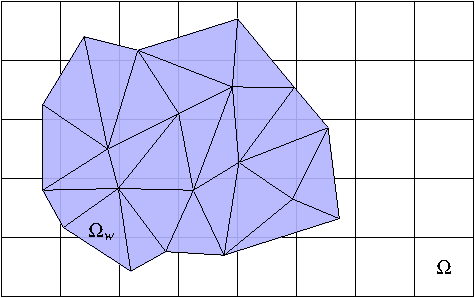
\includegraphics[width=.6\textwidth]{img/lagrangian/dual_pfem_mesh.pdf}
    \caption{Discretización espacial para el algoritmo PFEM de malla móvil}
    \label{pfem_dual_mesh}
\end{figure}

Se introduce una discretización de elementos finitos $\Omega_h$ para el subdominio $\Omega_w$, donde cada variable $\psi$ puede ser interpolada empleando las funciones base de los elementos finitos como
\begin{equation}
    \psi = \sum_a^{N_\Omega} N_a(\mathbf{x}) \psi_{a}
\end{equation}
donce $N_\Omega$ representa el número total de nodos en $\Omega_h$ y $\psi_a$ es el valor nodal de cada variable, ya sea una incógnita o cualquier variable característica. Se procede de igual modo para el dominio $\Omega$, donde están definidas las variables del terreno: la topografía y la rugosidad.


\subsection{Limitaciones del método}

Por un lado, dado que se están empleando las ecuaciones en variables primitivas, este método está especialmente indicado para resolver problemas en régimen subcrítico. No obstante, también es aplicable a problemas en régimen supercrítico, pues no hay ningún impedimento de estabilidad. La mayor limitación la encontramos en la presencia de discontinuidades, pues fácilmente se producirá una inversión de elementos. Este problema no se puede solucionar con un remallado, ya que los valores nodales resultarán en una interpolación errónea de las variables. A través de la figura \ref{pfem_shock} puede verse que la condición $CFL<1$ es un requisito para prevenir la inversión de elementos, incluso para esquemas de integración temporal implícitos.

\begin{figure}
    \centering
    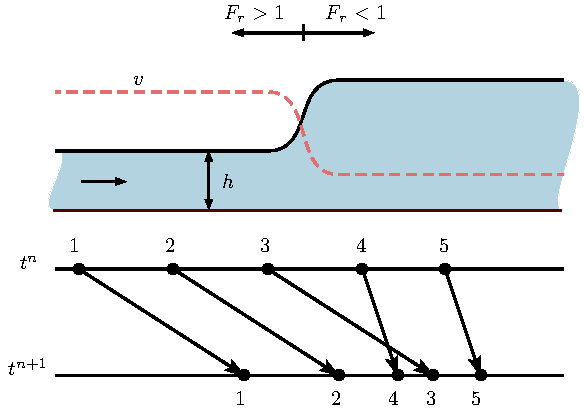
\includegraphics[width=.8\textwidth]{img/lagrangian/pfem_shock.pdf}
    \caption{Incompatibilidad que se presenta para el algoritmo de malla móvil ante la presencia de discontinuidades.}
    \label{pfem_shock}
\end{figure}



\section{Fixed mesh methods}

A diferencia del algoritmo tradicional PFEM, las partículas no coinciden con los nodos, sino que se mueven libremente sobre la malla de elementos finitos. Tiene la ventaja de no necesitar un remallado, pero el coste de definir una proyección para trasladar la información la malla de elementos finitos a las partículas.

En primer lugar, se define un conjunto de partículas que ocupan el dominio de aguas poco profundas. La densidad de partículas será tal que, habrá más partículas que elementos para el mismo dominio. Estas partícluas se desplazan transportando las propiedades intrínsecas (densidad, calado, velocidad, caudal, etc.). Después de la fase de desplazamiento, se proyectan las variables intrínsecas a la malla de elementos finitos, dando paso a la solución de un sistema de ecuaciones en un marco Lagrangiano. Es importante recalcar que para ello no se ha requierido ningún movimiento de la malla, pero sí la definición de una proyección. Esta primera proyección es trivial, ya que se emplea la interpolación de los elementos finitos.


%La información de la malla de elementos finitos se puede proyectar fácilmente a las partículas utilizando las funciones de forma. Sin embargo, la proyección de las partículas a la malla de elementos finitos requiere la definición de otra proyección.

%Estas partículas que se ha introducido, después de desplazarse, proyectan las variables intrínsecas a la malla de elementos finitos, dando paso a la solución de un sistema de ecuaciones en un marco Lagrangiano. Es importante recalcar que para ello no se ha requierido ningún movimiento de la malla, pero sí la definición de una proyección.

Un vez resuelto el sistema de ecuaciones, las partículas actualizan las variables características. Esta segunda proyección es un paso crítico, pues resulta necesario definir una proyección de los elementos a als partículas. Esta explicación resume brevemente el esquema de funcionamiento de una iteración no lineal. Usualmente, suele emplearse una sola iteración.

Igual que en el algoritmo de malla móvil, este esquema puede sufrir algunas variaciones, pues, en sentido estricto, se trata de un esquema implícito que requiere iterar entre en paso de convección y la resolución del sistema de ecuaciones. Dejamos el análisis del sistema de integración temporal para más adelante.


\subsection{Ecuaciones de gobierno}

A diferencia del algoritmo de malla móvil, los nodos reciben la información característica de la nueva configuración, sin que la malla se haya desplazado. Este hecho permite utilizar arbitrariamente un esquema Lagrangiano o Euleriano, independientemente de cómo se haya resuelto la convección. A la luz de esta consideración, es importante ver que la expresión de la conservación de la masa en un esquema Euelriano es trivial cuando se consideran variables conservativas. De este modo, consideramos la formulación Lagrangiana solamente en el balance de cantidad de movimiento. Otra posibilidad sería emplear las mismas ecuaciones de gobierno que en el caso de PFEM de malla móvil.

La aplicación de la regla de la cadena al operador convectivo nos lleva a la introducción de un nuevo término en el balande de cantidad de movimiento. Este término corresponde a la compresibilidad del flujo. Es importante recordad la analogía entre las ecuaciones de flujo compresible y las ecuaciones aguas poco profundas. Con tal de linealizar la solución del sistema de ecuaciones, se presentan tres vías que serán estudiadas:
\begin{itemize}
    \item Incluir el término de transporte compresible en el sistema de ecuaciones. Esta es la solución más consistente, sin embargo, la mas costosa ya que introduce una no linealidad y teŕminos que deben ser incluidos en la estabilización.
    \item Calcular el término compresible mediante la divergencia de los desplazamientos. Puesto que en la etapa de convección se calculan los desplazamientos, se dispone de los elementos necesarios para calcular la divergencia, modificando así la proyección de las variables intrínsecas a la malla de elementos finitos.
    \item Si la importancia relativa del presente término lo permite, omitirlo. Esta alternativa práctica, requiere la evaluación de aplicabilidad.
\end{itemize}


\subsection{Conclusiones}

Los métodos Lagrangianos presentan un esquema que permite un ahorro computacional. La gran ventaja que tienen es la facilidad para tratar el movimiento de la líne de costa o el avance de una inundación, evitando todos los problemas derivados de tener que incluir el dominio seco en el cálculo. El principal inconveniente de los métodos Lagrangianos está originado en que el campo de velocidades es discontínuo cuando hay un resalto hidráulico. Así como la discontinuidad que presenta la línea de costa queda resuelta de modo natural en los métodos Lagrangianos, la discontiuidad de los resaltos hidráulicos puede llevar a la inversión de elementos o proyecciones inadecuadas. Este aspecto necesita de técnicas específicas en los que la solución puede ser muy sensible al método utilizado, o puede ser poco robusta.

Por lo general, ante la presencia de resaltes hidráulicos, son preferibles los esquemas de integración temporal explícitos, frente a los implícitos. Puesto que la derivada no está definida en las discontinuidades, los esquemas semi-implícitos pueden llevar a soluciones que no convergen.




\section{Examples}



\section{Concluding remarks}


